\documentclass[12pt]{article}

\usepackage[margin=1in]{geometry}
\usepackage{amsmath,amsthm,amssymb}
\usepackage{nccmath}
\usepackage{mathtools}
\usepackage{mathrsfs}
\usepackage{enumitem}
\usepackage{physics}
\usepackage{tensor}
\usepackage{subcaption}

\usepackage{tikz}
\usetikzlibrary{calc,decorations.markings,patterns}

\newcommand{\magsq}[1]{\big|#1\big|^2}
\newcommand{\metric}{\mqty(1 & 0 & 0 & 0 \\ 0 & -1 & 0 & 0 \\ 0 & 0 & -1 & 0 \\ 0 & 0 & 0 & -1)}
\newcommand{\chrissym}[3]{\Gamma_{#2#3}^#1}
\newcommand{\partialg}[3]{\partial_{#1}g_{#2#3}}

\begin{document}

\title{Homework 2}
\author{Sean Ericson \\ Phys 610}
\maketitle

\section*{Problem 1}
Given the Lagrangian
\[ L = \frac{1}{2}mg_{ij}(x)\dot{x}^i\dot{x}^j, \]
and the definition of the christoffel symbols
\[ \chrissym{i}{j}{k} = \frac{1}{2}g^{il}\left(\partialg{k}{l}{j} + \partialg{j}{l}{k} - \partialg{l}{j}{k}\right), \]
we can start by taking derivatives of the Lagrangian:
\begin{align*}
    \pdv{L}{x^l} &= \frac{1}{2}m\pdv{g_{ij}(x)}{x^l}\dot{x}^i\dot{x}^j \\
    &= \frac{1}{2}m\partialg{l}{i}{j}\dot{x}^i\dot{x}^j
\end{align*}
\begin{align*}
    \pdv{L}{\dot{x}^l} &= \frac{1}{2}mg_{ij}\left(\pdv{\dot{x}^i}{\dot{x}^l}\dot{x}^j + \dot{x}^i\pdv{\dot{x}^j}{\dot{x}^l}\right) \\
    &= \frac{1}{2}mg_{ij}\left(\delta_{\;l}^i\dot{x}^j + \delta_{\;l}^j\dot{x}^i\right) \\
    &= \frac{1}{2}m\left(g_{lj}\dot{x}^j + g_{il}\dot{x}^i\right) \\
    &= mg_{li}\dot{x}^i
\end{align*}
\begin{align*}
    \dv{t}\pdv{L}{\dot{x}^l} &= \dv{t}\left(mg_{li}\dot{x}^i\right) \\
    &= m\dv{g_{li}}{t}\dot{x}^i + mg_{li}\dv{\dot{x}^i}{t} \\
    &= m \pdv{g_{li}}{x^j}\dv{x^j}{t}\dot{x}^i + mg_{li}\ddot{x}^i \\
    &= m \partialg{j}{l}{i}\dot{x}^i\dot{x}^j + mg_{li}\ddot{x}^i
\end{align*}
Now we can just plug these in to the Euler-Lagrange equation:
\begin{alignat*}{3}
    &         \quad & \dv{t}\pdv{L}{\dot{x}^l} &= \pdv{L}{x^l} \\
    &\implies \quad & m \partialg{j}{l}{i}\dot{x}^i\dot{x}^j + mg_{li}\ddot{x}^i &= \frac{1}{2}m\partialg{l}{i}{j}\dot{x}^i\dot{x}^j \\
    &\implies \quad & g_{li}\ddot{x}^i &= \left(\frac{1}{2}\partialg{l}{i}{j} - \partialg{j}{l}{i} \right)\dot{x}^i\dot{x}^j \\
    &         \quad &  &= -\frac{1}{2}\left(2\partialg{j}{l}{i} - \partialg{l}{i}{j}\right)\dot{x}^i\dot{x}^j \\
    &         \quad &  &= -\frac{1}{2}\left(\partialg{j}{l}{i} + \partialg{j}{l}{i} - \partialg{l}{i}{j}\right)\dot{x}^i\dot{x}^j \\
    &         \quad &  &= -\frac{1}{2}\left(\partialg{j}{l}{i} + \partialg{i}{l}{j} - \partialg{l}{i}{j}\right)\dot{x}^i\dot{x}^j \\
    &\implies \quad & \ddot{x}^i &= -\frac{1}{2}g^{il}\left(\partialg{k}{l}{j} + \partialg{j}{l}{k} - \partialg{l}{j}{k}\right)\dot{x}^j\dot{x}^k \\
    &         \quad &  &= -\chrissym{i}{j}{k}\dot{x}^j\dot{x}^k \\
    &\implies \quad & \ddot{x}^i + \chrissym{i}{j}{k}\dot{x}^j\dot{x}^k &= 0
\end{alignat*}
In the third-to-last line, the index relabeling $i \to j$ and $j \to k$ for contracted indices was used on the right-hand side.

\section*{Problem 2}
\begin{figure*}[h]
    \centering
    \begin{subfigure}[t]{0.3\textwidth}
        \centering
        \resizebox{150pt}{!}{
            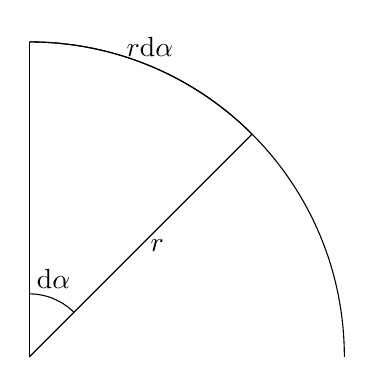
\begin{tikzpicture}
                \draw (0,4) arc (90:0:4);
                \draw (0,0)--(0,4);
                \draw (0,0)--({4*cos(45)},{4*sin(45)}) node[midway,right]{$r$};
                \draw (0,0.8) arc (90:45:0.8) node[midway,above]{$\dd\alpha$};
                \draw (0,4) arc (90:45:4) node[midway,above]{$r\dd\alpha$};
            \end{tikzpicture}
        }
        \caption{}
        \label{arclen_fig}
    \end{subfigure}%
    ~ 
    \begin{subfigure}[t]{0.3\textwidth}
        \centering
        \resizebox{150pt}{!}{
            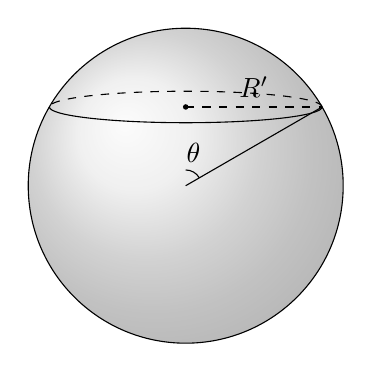
\begin{tikzpicture}
                \shade[ball color = gray!40, opacity = 0.4] (0,0) circle (2);
                \draw (0,0) circle (2);

                % Higher latitude
                \draw ({-sqrt(3)},1) arc (180:360:{sqrt(3)} and 0.2);
                \draw[dashed] ({sqrt(3)},1) arc (0:180:{sqrt(3)} and 0.2);
                \fill[fill=black] (0,1) circle (1pt);
                \draw[dashed] (0,1) -- node[above]{$R'$} ({sqrt(3)},1);

                % Angle
                \draw (0,0)--({sqrt(3)}, 1);
                \draw (0,0.2) arc (90:30:0.2) node[midway,above]{$\theta$};
            \end{tikzpicture}
        }
        \caption{}
        \label{latitude_fig}
    \end{subfigure}
    ~ 
    \begin{subfigure}[t]{0.3\textwidth}
        \centering
        \resizebox{150pt}{!}{
            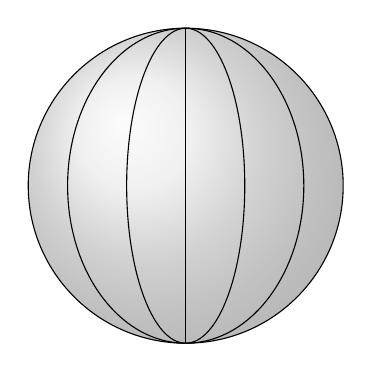
\begin{tikzpicture}
                \shade[ball color = gray!40, opacity = 0.4] (0,0) circle (2);
                \draw (0,0) circle (2);

                % Longitudes
                \draw (0,0) ellipse (0.75 and 2);
                \draw (0,0) ellipse (1.5 and 2);
                \draw (0,-2)--(0,2);
            \end{tikzpicture}
        }
        \caption{}
        \label{longitude_fig}
    \end{subfigure}
    \caption{(a) Arc length for a circle of radius $r$ and angle $\dd\alpha$. (b) A constant-$\theta$ circle on a 2-sphere. (c) Constant-$\phi$ circles on a 2-sphere.}
\end{figure*}

\begin{enumerate}[label=(\alph*)]
    \item As illustrated in Figure \ref{arclen_fig}, the arc length for a circle of radius $r$ and angle $\dd\alpha$ is $r\dd\alpha$. On a 2-sphere of radius $R$, paths of constant $\theta$ are circles of radius $R\sin\theta$ (Figure \ref{latitude_fig}), while paths of constant $\phi$ are circles of radius $R$ (Figure \ref{longitude_fig}). The $\hat{\theta}$ and $\hat{\phi}$ directions are orthogonal everywhere on the sphere, so the square of the total displacement is the sum of the squares of the displacements in either direction:
    \[ \dd s^2 = R^2\dd\theta^2 + R^2\sin^2\theta \dd\phi^2 \]
    \item The only nonzero christoffel symbols are
    \begin{align*}
        \chrissym{\theta}{\phi}{\phi} &= \frac{1}{2}g^{\theta l}\left(\partialg{\phi}{l}{\phi} + \partialg{\phi}{l}{\phi} - \partialg{l}{\phi}{\phi}\right) \\
        &= -\frac{1}{2}g^{\theta\theta}\partialg{\theta}{\phi}{\phi} \\
        &= -\frac{1}{2}\frac{1}{R^2}\pdv{\theta}R^2\sin^2\theta \\
        &= -\sin\theta\cos\theta \\
        \chrissym{\phi}{\theta}{\phi} &= \frac{1}{2}g^{\phi l}\left(\partialg{\phi}{l}{\theta} + \partialg{\theta}{l}{\phi} - \partialg{l}{\theta}{\phi}\right) \\
        &= \frac{1}{2}g^{\phi\phi}\partialg{\theta}{\phi}{\phi} \\
        &= \frac{1}{2}\frac{1}{R^2\sin^2\theta}\pdv{\theta}R^2\sin^2\theta \\
        &= \cot\theta \\
        &= \chrissym{\phi}{\phi}{\theta}
    \end{align*}
\end{enumerate}


\section*{Problem 3}
\begin{enumerate}[label=(\alph*)]
    \item 
    \[ \dv[2]{x^i}{s} = -\chrissym{i}{j}{k}\dot{x}^j\dot{x}^k \]
    \[ \dv[2]{\theta}{s} = \sin\theta\cos\theta\dot{\phi}^2 \]
    \[ \dv[2]{\phi}{s} = -\left(\chrissym{\phi}{\theta}{\phi}+\chrissym{\phi}{\phi}{\theta}\right)\dot{\theta}\dot{\phi} = -2\cot\theta\dot{\theta}\dot{\phi} \]
    \item
    \begin{alignat*}{3}
        &         \quad & \ddot{\phi} + 2\cot\theta\dot{\theta}\dot{\phi} &= 0  \\
        &\implies \quad & \sin^2\theta\ddot{\phi} + 2\sin\theta\cos\theta\dot{\theta}\dot{\phi} &= 0 \\
        &\implies \quad & \dv{t}\left(\sin^2\theta\dot{\phi}\right) &= 0 \\
    \end{alignat*}
    \begin{align*}
        \dv{t}\left(\dot{\theta}^2 + \sin^2\theta\dot{\phi}\right) &= 2\dot{\theta}\ddot{\theta} + 2\sin\theta\cos\theta\dot{\theta}\dot{\phi}^2 + 2\sin^2\theta\dot{\phi}\ddot{\phi} \\
        &= 2\sin\theta\cos\theta\dot{\theta}\dot{\phi}^2 + 2\sin\theta\cos\theta\dot{\theta}\dot{\phi}^2 - 4\sin\theta\cos\theta\dot{\theta}\dot{\phi}^2 \\
        &= 0
    \end{align*}
    \item
    \[ \tilde{L} = R^2\sin^2\theta\dot{\phi} \implies \dot{\phi} = \frac{1}{R^2\sin^2\theta} \]
    \[ u\cdot u = R^2\left(\dot{\theta}^2 + \sin^2\theta\dot{\phi}^2\right) = 1 \implies \dot{\theta}^2 = \frac{1}{R^2}\left(1 - \frac{L^2}{R^2\sin^2\theta}\right) \implies \dot{\theta} = \pm\frac{1}{R}\sqrt{1 - \frac{L^2}{R^2\sin^2\theta}} \]
    \[ \dv{\theta}{s} = \pm\frac{1}{R}\sqrt{1 - \frac{L^2}{R^2\sin^2\theta}} \implies \int\dd s = \pm\int \frac{R\dd\theta}{\sqrt{1 - \frac{L^2}{R^2\sin^2\theta}}} \]
    \item
    \[ z = R\cos\theta \implies \dd z = -R\sin\theta\dd\theta \]
    \[ z = R\sin I\cos\psi \implies \dd z = -R\sin I\sin\psi \]
    \[ \implies \psi = \cos^{-1}\frac{\cos\theta}{\sin I} \]
    \begin{align*}
        s &= \pm\int\frac{R\dd\theta}{\sqrt{1 - \frac{L^2}{R^2\sin^2\theta}}} \\
        &= \mp\int\frac{R\dd z}{\sqrt{R^2\sin^2\theta - L^2}} \\
        &= \mp\int\frac{R\dd z}{\sqrt{R^2\left(1 - \cos^2\theta\right) - L^2}} \\
        &= \mp\int\frac{R\dd z}{\sqrt{R^2 - L^2 - z^2}} \\
        &= \pm\int\frac{R^2\sin I\sin\psi\dd\psi}{\sqrt{R^2 - R^2\cos^2I - R^2\sin^2I\cos^2\psi}} \\
        &= \pm\int\frac{R\sin I\sin\psi\dd\psi}{\sqrt{1 - \cos^2I - \sin^2I\cos^2\psi}} \\
        &= \pm\int\frac{R\sin I\sin\psi\dd\psi}{\sqrt{\sin^2I - \sin^2I\cos^2\psi}} \\
        &= \pm\int\frac{R\sin\psi\dd\psi}{\sqrt{1 - \cos^2\psi}} \\
        &= \pm\int R\dd\psi \\
        &= R\psi + C \\
        \implies \qquad \frac{s-C}{R} &= \cos^{-1}\frac{\cos\theta}{\sin I} \\
        \implies \qquad \cos\theta &= \sin I\cos\frac{s-C}{R}
    \end{align*}

    \item Project the great circle onto a plane containing the $z$-axis. The result will be a (generalized) ellipse, hence motion in the $z$-direction will be sinusoidal. In this picture, $z$ is the $z$-component of the position on the geodesic in the 3-space in which the 2-sphere is embedded. $I$ and $\psi$ are related to the axis about which the geodesic ``rotates''.
\end{enumerate}


\section*{Problem 4}
\begin{align}
    \Delta_\rho g_{\mu\nu} &= \partial_\rho g_{\mu\nu} - \chrissym{\lambda}{\rho}{\mu}g_{\lambda\nu} - \chrissym{\lambda}{\rho}{\nu}g_{\mu\lambda} = 0 \\
    \Delta_\mu g_{\nu\rho} &= \partial_\mu g_{\nu\rho} - \chrissym{\lambda}{\mu}{\nu}g_{\lambda\rho} - \chrissym{\lambda}{\mu}{\rho}g_{\nu\lambda} = 0 \\
    \Delta_\nu g_{\rho\mu} &= \partial_\nu g_{\rho\mu} - \chrissym{\lambda}{\nu}{\rho}g_{\lambda\mu} - \chrissym{\lambda}{\nu}{\mu}g_{\rho\lambda} = 0
\end{align}
$(1) - (2) - (3)$:
\begin{align*}
    \partial_\rho g_{\mu\nu} - \partial_\mu g_{\nu\rho} - \partial_\nu g_{\rho\mu} + 2\chrissym{\lambda}{\mu}{\nu}g_{\rho\lambda} = 0 \\
    \implies g_{\rho\lambda}\chrissym{\lambda}{\mu}{\nu} = \frac{1}{2}\left(\partial_\nu g_{\rho\mu} + \partial_\mu g_{\nu\rho} - \partial_\rho g_{\mu\nu} \right) \\
    \implies \chrissym{\rho}{\mu}{\nu} = \frac{1}{2} g^{\rho\lambda}\left(\partial_\nu g_{\lambda\mu} + \partial_\mu g_{\nu\lambda} - \partial_\lambda g_{\mu\nu}\right)
\end{align*}

\end{document}